\documentclass[a4paper,12pt]{article}
\usepackage[utf8]{inputenc}
\usepackage[russian]{babel}
\usepackage{graphicx}
\usepackage{geometry}
\usepackage[colorlinks=true, urlcolor=blue]{hyperref}
\geometry{a4paper, margin=2cm}
\usepackage{setspace}
\onehalfspacing

\begin{document}
	
	\begin{center}
		\Large\textbf{Предложение проекта: БПЛА - беспилотный летательный аппарат}
	\end{center}
	
	\vspace{0.5cm}
	
	\textbf{Команда:}\\
	Шелонин Арсений Карленович \texttt{(shelonin.ak@phystech.edu}),\\
	Себелев Максим Максимович \texttt{(sebelev.mm@phystech.edu)},\\
	Дернович Арсений Андреевич
	\texttt{(dernovich.aa@phystech.edu)} 
	
	\vspace{0.5cm}
	
	\textbf{Цель проекта:} спроектировать и изготовить беспилотный летательный аппарат (FPV дрон) на пульте дистанционного управления, пригодного для использования в военно-гумманитарных :) целях, требующий для изготовления минимальных вложений денежных средств. Боевой задачей дрона является отвлечение вражеского ПВО - оценочная стоимость дрона в десятки раз меньше стоимости запуска ракеты ПВО.
	
	\vspace{0.5cm}
	
	\textbf{Задачи проекта:}
	\begin{itemize}
		\item подобрать наиболее финансово демократичный в меру прочный материал обшивки корпуса БПЛА, пригодный для совершения дальних полетов;
		\item разработать собственную систему управления дроном с использованием датчиков GPS, акселерометра и видео-камеры;
		\item собрать опытный образец;
		\item оценить и сравнить стоимости с учетом и без конвейерного производства;
		\item провести летные испытания;
	\end{itemize}
	
	\vspace{0.5cm}
	
	\textbf{Существующие аналоги:}
	\begin{enumerate}
		\item \textit{fpv-дрон "Архангел"}\\
		Стоимость и ТТХ (тактико-технические характеристики):\\
		\href{https://www.tadviser.ru/index.php/%D0%A1%D1%82%D0%B0%D1%82%D1%8C%D1%8F:%D0%92%D0%BE%D0%B5%D0%BD%D0%BD%D1%8B%D0%B5_%D0%B4%D1%80%D0%BE%D0%BD%D1%8B_%D0%B2_%D0%A0%D0%BE%D1%81%D1%81%D0%B8%D0%B8}{Tadviser: Архангел}
		\item \textit{fpv-дрон "Черника-2"}\\
		Стоимость и ТТХ (тактико-технические характеристики):\\
		\href{https://www.tadviser.ru/index.php/%25D0%25A1%25D1%2582%25D0%25B0%25D1%2582%25D1%258C%25D1%258F:%25D0%2592%25D0%25BE%25D0%25B5%25D0%25BD%25D0%25BD%25D1%258B%25D0%25B5_%25D0%25B4%25D1%2580%25D0%25BE%25D0%25BD%25D1%258B_%25D0%25B2_%25D0%25A0%25D0%25BE%25D1%2581%25D1%2581%25D0%25B8%25D0%25B8}{Tadviser: Черника-2}
		
	\end{enumerate}
	

	\section{Планы на итоговый отчет}
	
	Подробное исследование преимуществ и недостатков проектной версии и приведенных аналогов будет произведено в итоговом отчете. \\
	На данный момент оценочная стоимость примерно 5000 рублей. Такую дешевизну обуславливает малая стоимость корпуса и деталей. Более подробно все экономические аспекты будут так же оценены в итоговом отчете.	

	\vspace{1cm}
	
	\textbf{Готовые разработки проекта:}
	
	\begin{center}
		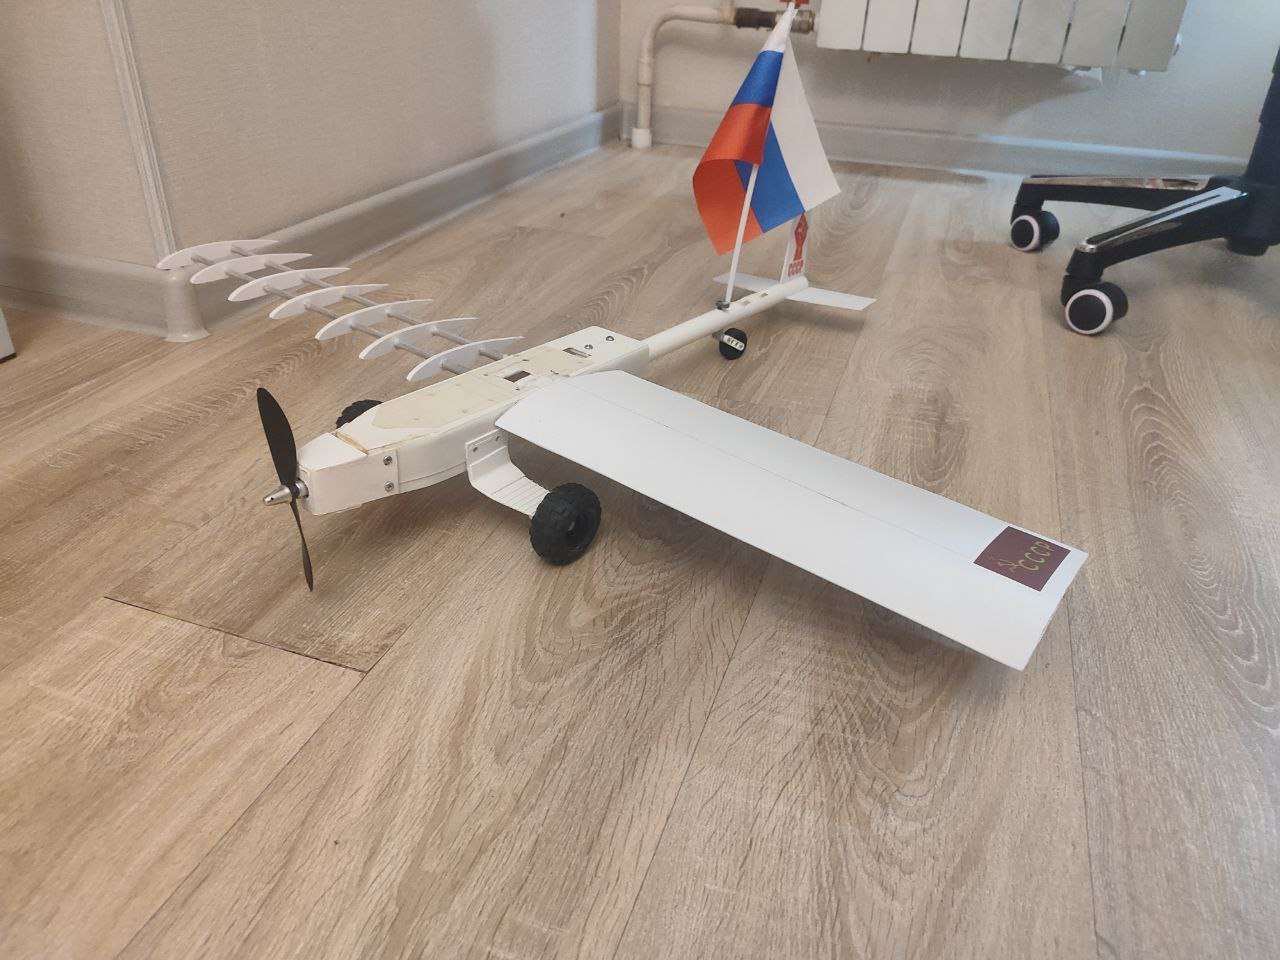
\includegraphics[width=0.8\textwidth]{main_model.jpg}
		\begin{center}
			\begin{tabular}{c}
				Корпус дрона\\			
			\end{tabular}
		\end{center}
		
	\end{center}
	
	\begin{center}
		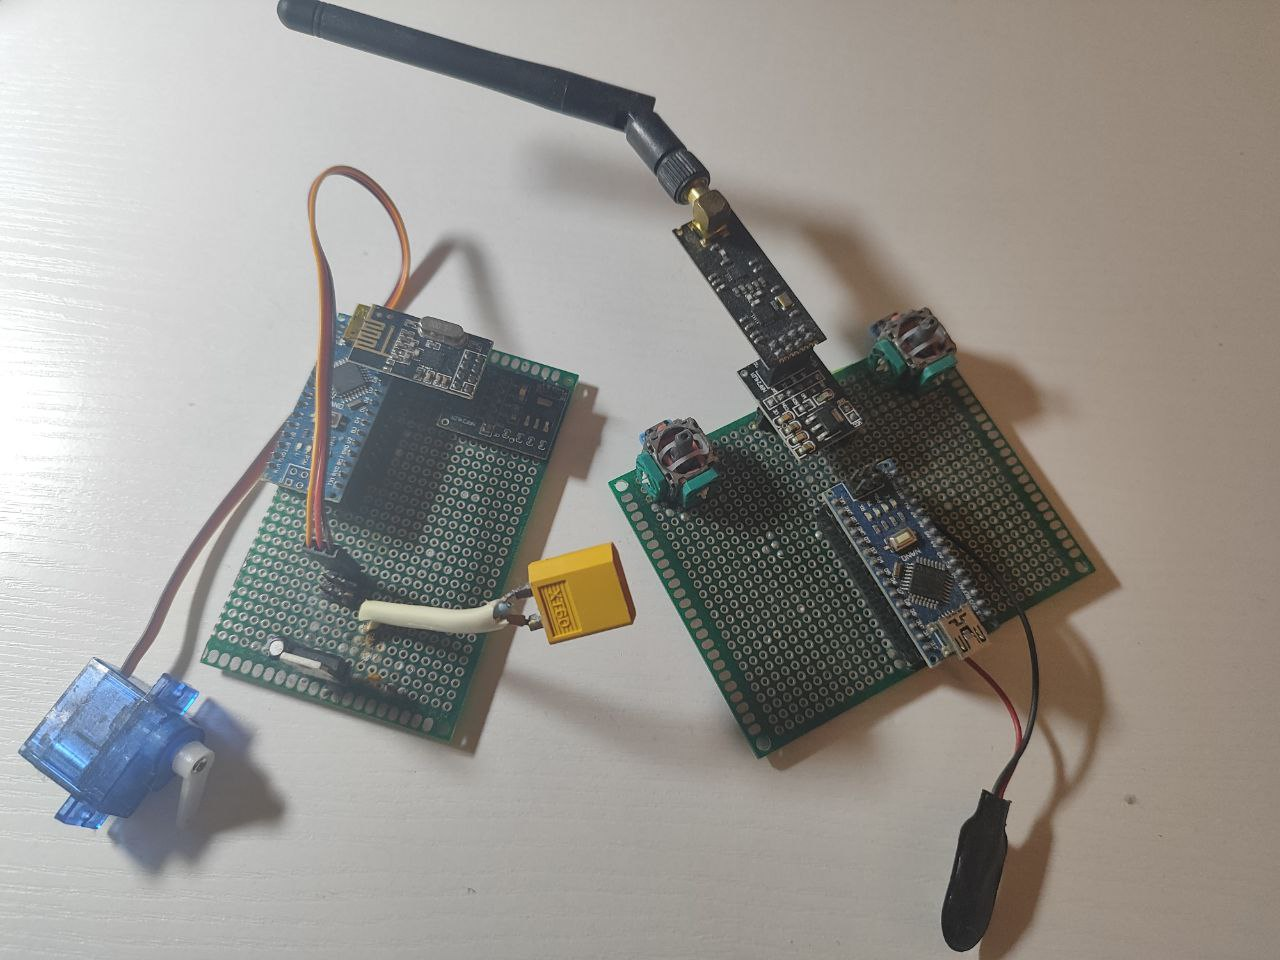
\includegraphics[width=0.8\textwidth]{plats.jpg}
		\begin{center}
			\begin{tabular}{c}
				Главные платы,\\предназначенные для управления дроном (мозги)
			\end{tabular}
		\end{center}
		
	\end{center}
	
	\begin{center}
		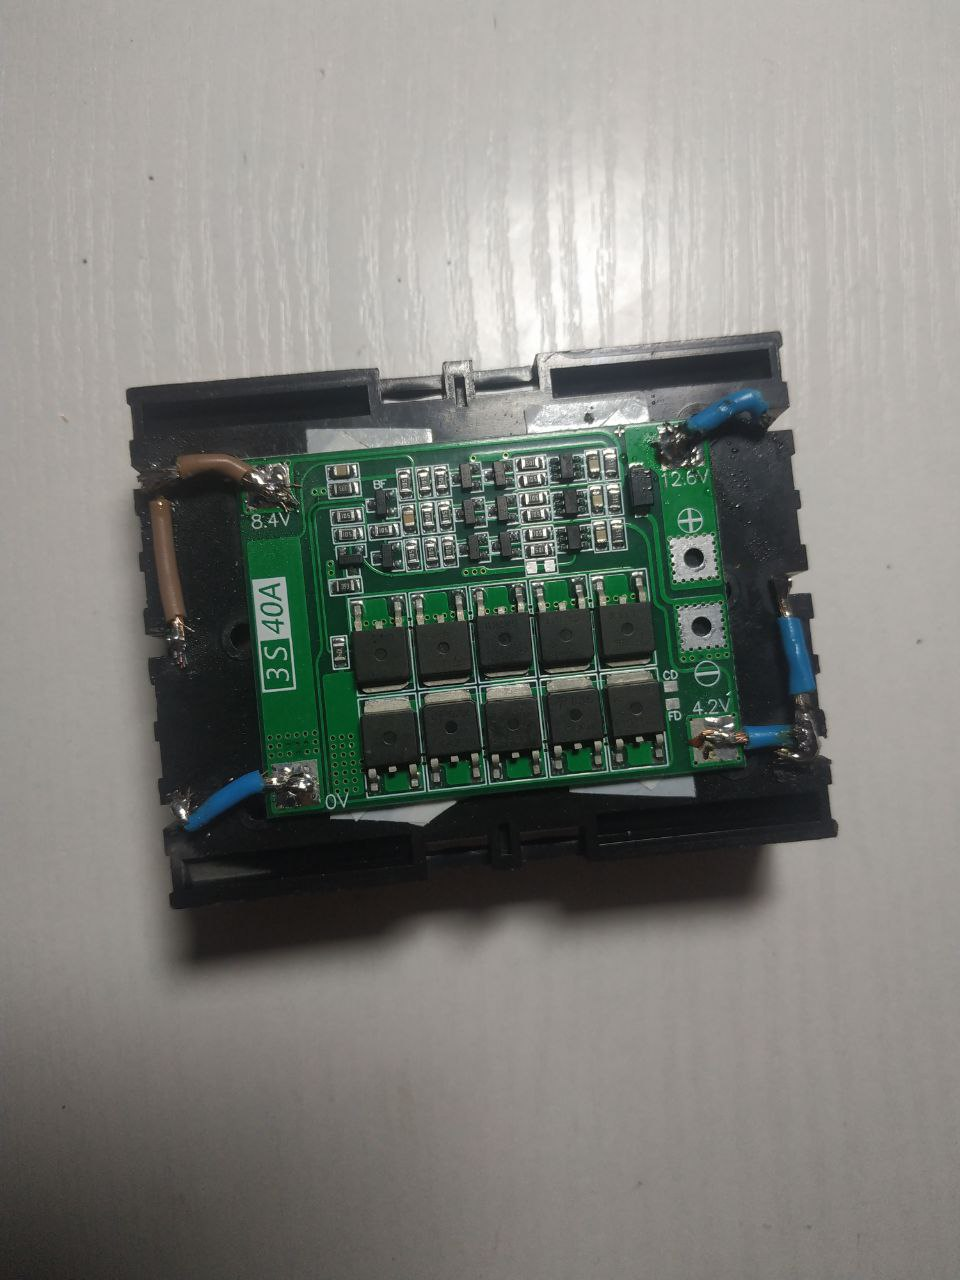
\includegraphics[width=0.8\textwidth]{balans.jpg}
		\begin{center}
			\begin{tabular}{c}
				Плата балансировки литий-ионных батарей\\(BMS 3S 40A)\\
			\end{tabular}
		\end{center}
		
	\end{center}
		

	
\end{document}